\documentclass[tikz, border=8pt]{standalone}
\usepackage{xcolor}
\usetikzlibrary{arrows.meta, positioning, shapes.geometric, calc, fit}
% ============================================================
% Shared style definitions for the DarwinsRNAHunt methods figures.
% \input this file from each diagram's preamble (after \usepackage{xcolor}
% and \usetikzlibrary{...}) so colours/styles stay consistent everywhere.
%
% Visual grammar used throughout:
%   - white box, single border   = external / raw resource
%   - white box, double border   = curated data artifact (output of a section)
%   - coloured box, single border = an internal processing step
%   - coloured/white, dashed border = Snakemake checkpoint (dynamic re-evaluation)
%   - white box, short-dashed border = static external file (not produced by the pipeline)
% ============================================================

% ---------- category colours (ColorBrewer Set3-style) ----------
\definecolor{catDefine}{HTML}{FFFFFF}
\definecolor{catSelect}{HTML}{FFFFFF}
\definecolor{catAcquire}{HTML}{FFFFFF}
\definecolor{catLocalize}{HTML}{FFFFFF}
\definecolor{catExtract}{HTML}{FFFFFF}
\definecolor{catCombine}{HTML}{FFFFFF}
\definecolor{catCluster}{HTML}{FFFFFF}
\definecolor{catModel}{HTML}{FFFFFF}
\definecolor{catValidate}{HTML}{FFFFFF}
\definecolor{catReport}{HTML}{FFFFFF}

% ---------- Kea Palette (defined for optional future restyling; unused for now) ----------
\definecolor{keaGreen}{HTML}{6C803A}
\definecolor{darkBrown}{HTML}{7B5C34}
\definecolor{lightBrown}{HTML}{AB7C47}
\definecolor{keaYellow}{HTML}{CCAE42}
\definecolor{keaOrange}{HTML}{D73202}
\definecolor{charcoal}{HTML}{272318}
\definecolor{lightGrey}{HTML}{D3CDBF}

\tikzset{
    font=\fontsize{7}{8}\selectfont,
    >={Latex[length=2mm,width=1.4mm]},
    every path/.style={thick},
    % internal processing step
    stage/.style={rectangle, rounded corners=2pt, draw=black, thin,
        minimum height=1.05cm, text width=3.6cm, align=center, inner sep=3pt},
    % external / raw resource (input)
    res/.style={rectangle, rounded corners=2pt, draw=black, thin, fill=white,
        minimum height=1cm, text width=4.2cm, align=center, inner sep=3pt},
    % static external file, not produced by this pipeline
    ext/.style={rectangle, rounded corners=2pt, draw=black!55, dash pattern=on 2.2pt off 1.6pt,
        thin, minimum height=0.85cm, text width=3.1cm, align=center, fill=white,
        font=\fontsize{6.3}{7.3}\selectfont, inner sep=2.5pt},
    % Snakemake checkpoint modifier (combine with stage/res)
    ckpt/.style={dashed, line width=0.9pt},
    % deliverable / output-artifact modifier: crosses a section boundary
    deliver/.style={double, double distance=1.2pt, line width=0.85pt},
    lbl/.style={font=\fontsize{8.5}{9.5}\bfseries\selectfont},
    sublbl/.style={font=\fontsize{7}{8}\itshape\selectfont},
    node distance=0.55cm and 2.6cm
}


\begin{document}
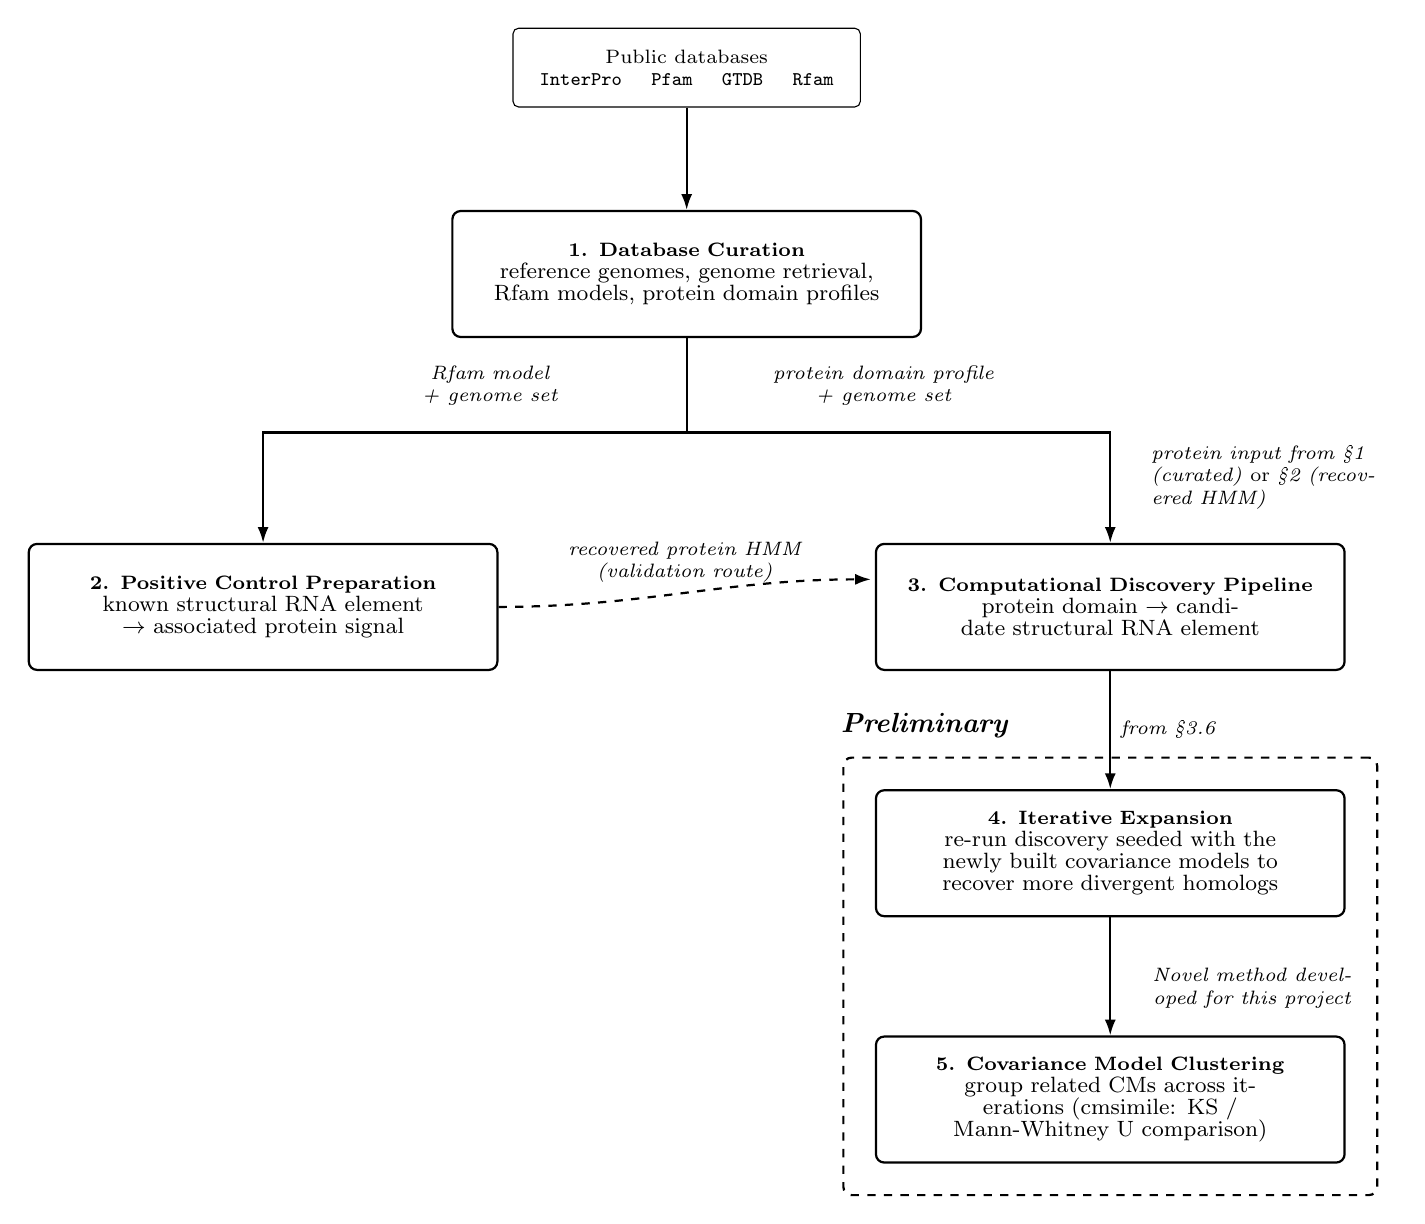
\begin{tikzpicture}[
    section/.style={rectangle, rounded corners=3pt, draw=black, thick,
        minimum height=1.6cm, text width=5.6cm, align=center, inner sep=5pt},
]

\node[res] (dbs) at (0,0) {Public databases\\\texttt{InterPro} \quad \texttt{Pfam} \quad \texttt{GTDB} \quad \texttt{Rfam}};

\node[section, fill=catDefine!35, below=1.3cm of dbs] (curation)
    {\textbf{1. Database Curation}\\\footnotesize reference genomes, genome retrieval, Rfam models, protein domain profiles};

\node[section, fill=catValidate!35, below left=2.6cm and -0.6cm of curation] (posctrl)
    {\textbf{2. Positive Control Preparation}\\\footnotesize known structural RNA element $\rightarrow$ associated protein signal};

\node[section, fill=catLocalize!35, below right=2.6cm and -0.6cm of curation] (discovery)
    {\textbf{3. Computational Discovery Pipeline}\\\footnotesize protein domain $\rightarrow$ candidate structural RNA element};

\draw[->] (dbs) -- (curation);
\draw[->] (curation.south) -- ++(0,-1.2cm) -| (posctrl.north);
\draw[->] (curation.south) -- ++(0,-1.2cm) -| (discovery.north);
\node[sublbl, text width=3.2cm, align=center] at ($(curation.south)+(-2.5,-0.6cm)$) {Rfam model\\+ genome set};
\node[sublbl, text width=3.2cm, align=center] at ($(curation.south)+(2.5,-0.6cm)$) {protein domain profile\\+ genome set};

\draw[->, dashed] (posctrl.east) to[out=0, in=180]
    node[midway, above, sublbl, text width=3.6cm, align=center]
    {recovered protein HMM\\(validation route)} ($(discovery.west)+(-0.05,0.35)$);

\node[sublbl, above right=0.3cm and -2.6cm of discovery, text width=3.0cm, align=left]
    {protein input from \S1 (curated) \emph{or} \S2 (recovered HMM)};

\node[section, fill=catModel!30, below=1.5cm of discovery] (iterexp)
    {\textbf{4. Iterative Expansion}\\\footnotesize re-run discovery seeded with the newly built covariance models to recover more divergent homologs};

\node[section, fill=catCluster!30, below=1.5cm of iterexp] (cmcluster)
    {\textbf{5. Covariance Model Clustering}\\\footnotesize group related CMs across iterations (cmsimile: KS / Mann-Whitney U comparison)};

\draw[->] (discovery) -- (iterexp) node[midway, right, sublbl, text width=2.6cm] {from \S3.6};
\draw[->] (iterexp) -- (cmcluster);
\node[sublbl, text width=3.2cm, align=center] at ($(cmcluster.north)+(+1.8,+0.6cm)$) {Novel method developed for this project};

\node[draw=black, dashed, rounded corners=3pt, inner sep=0.4cm,
      fit=(iterexp)(cmcluster),
      label={[font=\bfseries\itshape, anchor=south west, xshift=-0.15cm, yshift=0.1cm]north west:Preliminary}] {};

\end{tikzpicture}
\end{document}
